\begin{frame}
\frametitle{Uso de la biblioteca de Clingo}

\begin{itemize}
	\item<1-> Permite embeber código en Lua (por defecto) o en Python (recompilándolo).
	
	\vspace{0.5em}
	
	\item<2-> Los dos lenguajes comparten la interfaz de funciones, variables, 
	métodos, etc.
	
	\vspace{0.5em}
	
	\item<3-> Para este proyecto se ha usado \textcolor{UDCpink}{Lua}.
\end{itemize}

\vspace{0.5em}

\pause[4]

\centering
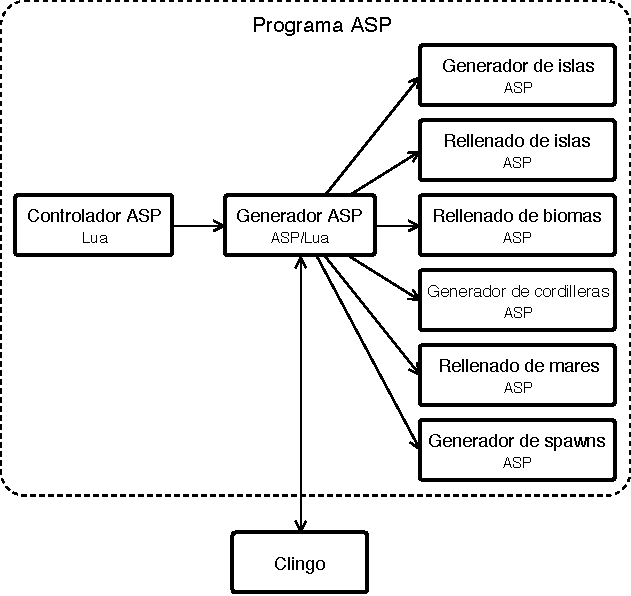
\includegraphics[width=0.4\textwidth]{images/arquitectura-final.pdf}
\end{frame}